\documentclass[fsharpNotes.tex]{subfiles}
\graphicspath{ {./figures/} }

\begin{document}
\chapter{Solving problems by writing a program}
\label{chap:quickStartGuide}

\abstract[figures/quickStartGuide]{
  In this chapter, you will find a quick introduction to several essential programming constructs with several examples that you can try on your computer using the \lstinline[language=console]{dotnet} command in your console. All constructs will be discussed in further detail in the following chapters. In this chapter, you will get a peek at:
  \begin{itemize}
  \item How to execute an F\# program.
  \item How to perform simple arithmetic using F\#.
  \item What types are and why they are important.
  \item How to write to and obtain written input from the user.
  \item How to perform conditional execution of code.
  \item How to define functions.
  \item How to repeat code without having to rewrite them.
  \item How to add textual comments to help yourself and other programmers understand your programs.
  \end{itemize}
}

Programming is the art of solving problems by writing a program to be executed by a computer. For example, to solve the following problem,
%
\begin{task}{probl:sumInteger}
  What is the sum of 357 and 864?
\end{task}
%
we have written the program shown in \Cref{quickStartSum}.
%
\fs{quickStartSum}{A script to add 2 numbers and print the result to the console.}
%
In this book, we will show many programs, and for most, we will also show the result of executing the programs on a computer. \Cref{quickStartSum} shows both our program and how this program is executed on a computer. In the listing, we see our program was saved as a script in a file called \lstinline[language=console]{quickStartSum.fsx}, and in the console (also known as the terminal and the command-line) we executed the program by typing the command \lstinline[language=console]|dotnet fsi quickStartSum.fsx|. The result is then printed by the computer to the console as \lstinline{1221}. The colors are not part of the program but have been added to make it easier for us to identify different syntactical elements of the program.

The program consists of several lines. Our listing shows line numbers to the left. These are not part of the program but added for ease of discussion, since the order in which the lines appear the program matters. In this program, each line contains \idx[expression]{expressions}, and this program has \keyword{let}-, \keyword{do}-expressions, and an addition. \keyword{let}-expressions defines aliases, and \keyword{do}-expressions defines computations. \keyword{let} and \keyword{do} are examples of \idx[keyword]{keywords}, and \lexeme{+} is an example of an \idx{operator}. Keywords, operators, and other sequences of characters, which F\# recognizes are jointly called \idx[lexeme]{lexemes}.

Reading the program from line~\ref{quickStartSumA}, the first expression we encounter is \lstinline|let a = 357|. This is known as a \idx{let-binding} in F\# and defines the equivalence between the name \lstinline{a} and the value \lstinline{357}. F\# does not accept a keyword as a name in a \keyword{let}-bindings. The consequence of this line is that in later lines there is no difference between writing the name \lstinline{a} and the value \lstinline{357}. Similarly in line~\ref{quickStartSumB} the value 864 is bound to the name \lstinline|b|. In contrast, line~\ref{quickStartSumC} contains an addition and a \keyword{let}-expression. It is at times useful to simulate the execution the computer does in a step-by-step manner by replacement:
\begin{quote}
  \lstinline{let c = a + b} $\quad\rightsquigarrow\quad$  \lstinline{let c = 357 + 864}  $\quad\rightsquigarrow\quad$  \lstinline{let c = 1221}
\end{quote}
Thus, since the expression on the right-hand side of the equal sign is evaluated, the result of line~\ref{quickStartSumC} is that the name \lstinline{c} is bound to the value \lstinline{1221}.

Line~\ref{quickStartSumPrintfn} has a \keyword{do}-expression is also called a \idx{do-binding} or a \idx[statement]{statements}. In this \keyword{do}-binding, the  \idx[printfn@\lstinline{printfn}]{\lstinline{printfn}} \idx{function} \lstinline{printfn} is called with 2 arguments, \lstinline{"%A"}%
  and \lstinline{c}. All functions return values, and \lstinline|printfn| the value 'nothing', which is denoted \idx[{()}@\lstinline{()}]{\lexeme{()}}. This function is very commonly used but also very special since it can take any number of arguments and produces output to the console. We say that ``the output is printed to the screen''. The first argument is called the \idx{formatting string} and describes, what should be printed and how the remaining arguments if any, should be formatted. In this case, the value \lstinline{c} is printed as an integer followed by a newline. Notice that in contrast to many other languages, F\# does not use parentheses to frame the list of function arguments, nor does it use commas to separate them.

\section{Executing F\# programs on a computer}
The main purpose of writing programs is to make computers execute or run them. F\# has two modes of execution, \idx[interactive mode]{interactive} and \idx[compile mode]{compiled}. Interactive mode allows the user to interact with F\# as a dialogue: The user writes statements, and F\# responds immediately. If a program has been saved as a file as in \Cref{quickStartSum} we do not need to rewrite the complete program every time we wish to execute it but can give the file as input to the F\#'s interactive mode as demonstrated in \Cref{quickStartSum}. Interactive mode is well suited for small experiments or back-of-an-envelope calculations, but not for programming in general, since each line is interpreted anew every time the program is run. In contrast, in compile mode, dotnet interprets the content of a source file once, and writes the result to disk, such that every when the user wishes to run the program, the interpretation step is not performed. For large programs, this can save considerable time. In the first chapters of this book, we will use interactive mode, and compile mode will be discussed in further detail in \Cref{chap:projects}.

An interactive session is obtained by starting the console, typing the \lstinline[language=console]{fsharpi} command, typing the lines of the program, and ending the script-fragment with \lexeme{;;}. The dialogue in \Cref{interactiveSession} demonstrates the workflow. What the user types has been highlighted by a \tikzmark{tl}box\tikzmark{br}\FrameArea{tl}{br}.
%
\begin{codeNOutput}[label=interactiveSession,
  top=-5pt,
  bottom=-5pt,
  left=-2pt,
  right=-2pt,
]{: An interactive session.}
  \begin{lstlisting}[language=console,escapechar=§]
$ §\tikzmark{lst1_5-tl}§dotnet fsi§\tikzmark{lst1_5-br}§

Microsoft (R) F# Interactive version 12.0.0.0 for F# 6.0
Copyright (c) Microsoft Corporation. All Rights Reserved.

For help type #help;;

> §\tikzmark{lst1_4-tl}§let a = 3§\tikzmark{lst1_1-start}§
- do printfn "%A" a;;§\tikzmark{lst1_4-br}§§\tikzmark{lst1_1-end}§
3§\tikzmark{lst1_2-start}§
val a : int = 3 §\tikzmark{lst1_2-align}§
val it : unit = ()
§\tikzmark{lst1_2-end}§
> §\tikzmark{lst1_6-tl}§#quit;;§\tikzmark{end_3}§§\tikzmark{lst1_6-br}§
\end{lstlisting}%$
\FrameArea{lst1_4-tl}{lst1_4-br}%
\FrameArea{lst1_5-tl}{lst1_5-br}%
\FrameArea{lst1_6-tl}{lst1_6-br}%
\end{codeNOutput}%
%
We see that after typing \lstinline[language=console]{fsharpi}, the program starts by stating details about itself. Then F\# writes \lstinline{>} indicating that it is ready to receive commands. The user types \lstinline{let a = 3} and presses \lstinline[language=console]{enter}, to which the interpreter responds with \lstinline{-}. This indicates that the line has been received, that the script fragment is not yet completed, and that it is ready to receive more input. When the user types \lstinline{do printfn "%A" a;;} %
followed by \lstinline[language=console]{enter}, then by \lexeme{;;} the interpreter knows that the script-fragment is completed, it interprets the script-fragment, responds with \lstinline{3} and some extra information about the entered code, and with \lstinline{>} to indicate that it is ready for more script-fragments. The interpreter is stopped when the user types \lstinline[language=console]{#quit;;}. It is also possible to stop the interpreter by typing \lstinline[language=console]{ctrl-d}.

The interactive session results in extra output on the \idx{type inference} performed. In \Cref{interactiveSession}, F\# states that the name \lstinline{a} has \idx{type} \keyword{int} and the value \lstinline{3}. Likewise, the \keyword{do} statement F\# refers to by the name \lstinline{it}, and it has the type \keyword{unit} and value \lexeme{()}. Types are very important to F\# since they define how different program pieces fit together like lego bricks. They are a key ingredient for finding errors in programs, also known as \idx{debugging}, and much of the rest of this book is concerned with types.

Instead of running \lstinline[language=console]{fsharpi} interactively, we can write the script-fragment from \Cref{interactiveSession} into a file, here called \lstinline[language=console]{gettingStartedStump.fsx}. This file can be interpreted directly by \lstinline[language=console]{dotnet fsi} as shown in \Cref{commandlineInterpreter}.
%
\begin{codeNOutput}[label=commandlineInterpreter,
  top=-5pt,
  bottom=-5pt,
  left=-2pt,
  right=-2pt,
]{: Using the interpreter to execute a script.}
\begin{lstlisting}[language=console,escapechar=§]
$ §\tikzmark{lst2_1-tl}§dotnet fsi gettingStartedStump.fsx§\tikzmark{lst2_1-br}§
3
\end{lstlisting}%$
\FrameArea{lst2_1-tl}{lst2_1-br}%
\end{codeNOutput}
%
Notice that in the file, \lexeme{;;} is optional. In comparison to \Cref{interactiveSession}, we see that the interpreter executes the code and prints the result on screen without the extra type information.

Files are important when programming, and F\# and the console interprets files differently by the filename's suffix. A filename's suffix is the sequence of letters after the period in the filename. Generally, there are two types of files: \idx{source code} and compiled programs. Until \Cref{chap:projects}, we will concentrate on script files, which are source code, written in human-readable form using an editor, and has \texttt{.fsx} or \texttt{.fsscript} as suffix. In \Cref{tab:suffix} is a complete list of possible suffixes used by F\#.

\begin{table}
  \centering
  \begin{tabular}{|l|l|l|}
    \hline
    Suffix & Human readable & Description\\
    \hline
    \lstinline[language=console]|.fs| & Yes & An \idx{implementation file}, e.g., \lstinline[language=console]|myModule.fs|\\
    \lstinline[language=console]|.fsi| & Yes & A \idx{signature file}, e.g., \lstinline[language=console]|myModule.fsi|\\
    \lstinline[language=console]|.fsx| & Yes & A \idx{script file}, e.g., \lstinline[language=console]|gettingStartedStump.fsx|\\
    \lstinline[language=console]|.fsscript| & Yes & Same as \lstinline[language=console]|.fsx|, e.g., \lstinline[language=console]|gettingStartedStump.fsscript|\\
    \hline
    \lstinline[language=console]|.dll| & No & A \idx{library file}, e.g., \lstinline[language=console]|myModule.dll|\\
    \lstinline[language=console]|.exe| & No & A stand-alone \idx{executable file}, e.g., \lstinline[language=console]|gettingStartedStump.exe|\\
    \hline
  \end{tabular}
  \caption{Suffixes used, when programming F\#.}
  \label{tab:suffix}
\end{table}

\section{Values have types and types reduce the risk of programming errors}
Types are a central concept in F\#. In the script \ref{quickStartSum} we bound values of integer type to names. There are several different integer types in F\#, here we used the one called \keyword|int|. The values were not \idx[type declaration]{declared} to have these types, instead the types were \idx[type inference]{inferred} by F\#. Typing these bindings line by line in an interactive session, we see the inferred types as shown in \Cref{typeInference}.
%
\fsOutput{typeInference}{Inferred types are given as part of the response from the interpreter.}
%
The interactive session displays the type using the \idx[val@\keyword{val}]{\keyword{val}} keyword followed by the name used in the binding, its type, and its value. Since the value is also returned, the last \lstinline|printfn| statement is superfluous. Notice that \lstinline{printfn} is automatically bound to the name \idx[it@\lstinline{it}]{\lstinline{it}} of type \keyword{unit} and value \idx[{()}@\lstinline{()}]{\lexeme{()}}. F\# insists on binding all statements to values, and in lack of an explicit name, it will use \lstinline{it}. Rumor has it that \lstinline{it} is an abbreviation for "irrelevant".

In mathematics, types are also an important concept. For example, a number may belong to the set of natural $\Nat$, integer $\Int$, or real numbers, where all 3 sets are infinitely large and $\Nat\subset\Int\subset\Re$ as illustrated in \Cref{fig:numbers}.
\begin{figure} % We want the figure on the first page with the chapter title
  \centering
  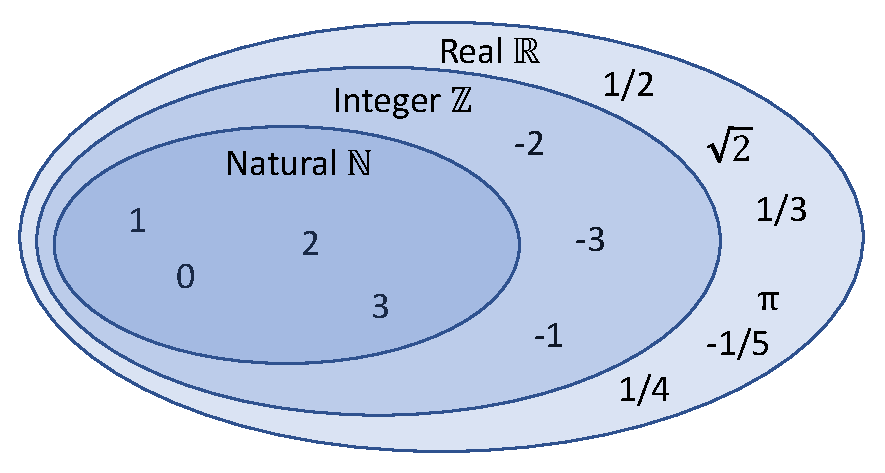
\includegraphics[width=0.6\textwidth]{numbers}
  \caption{In mathematics, the sets of natural, integer, and real numbers are each infinitely large, and real contains integers which in turn contains the set of natural numbers.}
  \label{fig:numbers}
\end{figure}
For many problems, working with infinite sets is impractical, and instead, a lot of work in the early days of the computer's history was spent on designing finite sets of numbers, which have many of the properties of their mathematical equivalent, but which also are efficient for performing calculations on a computer. For example, the set of integers in F\# is called \keyword{int} and is the set $\{\numprint{-2147483648} \ldots \numprint{2147483647}\}$.

Types are also important when programming. For example, a the \lstinline{string} \lstinline{"863"} and the \lstinline{int} \lstinline{863} may conceptually be identical but they are very different in the computer. F\# is very picky about types, and generally does not allow types to be mixed, as demonstrated in the interactive session in \Cref{typeInferenceError}.
%
\fsOutput{typeInferenceError}{Mixing types is often not allowed.}
%
In this example, we see that adding a string to an integer results in an error. The \idx{error message} contains much information. First, it illustrates where dotnet could not understand the input by \lstinline{------------^}. Then it repeats where the error is found as \lstinline[language=console]{/User/.../src/stdin(3,13)}, which means that \lstinline[language=console]{dotnet} was started in the directory \lstinline[language=console]{/User/.../src/}, the input was given on the standard-input meaning the keyboard, and the error was detected on line 3, column 13. Then  F\# gives the error number and a description of the error. Error numbers are an underdeveloped feature in F\# and should be ignored. However, the verbal description often contains useful information for correcting the program. Here, we are informed that there is a type mismatch in the expression. The reason for the mismatch is that since \lstinline{a} is an integer, then the \lexeme{+} operator must be integer addition, and thus for the expression to be executable, \lstinline{b} can only be an integer.

\section{Organizing often used code in functions}
\lstinline{printfn} is an example of a built-in function, and very often we wish to define our own. For example, in longer programs, some code needs to be used in several places, and defining functions to \idx{encapsulate} such code can be a great advantage for reducing the length of code, debugging, and writing code, which is easier to understand by other programmers. A function is defined using a \keyword{let}-binding. For example, to define a function, which takes two integers as input and returns their sum, we write
%
\begin{codeNOutput}[label=sumFunction,
  top=-5pt,
  bottom=-5pt,
  left=-2pt,
  right=-2pt,
]{: Defining the function \lstinline{sum}}
\begin{lstlisting}
let sum x y =
  x + y
\end{lstlisting} 
\end{codeNOutput}
%
What this means is that we bind the name \lstinline{sum} as a function, which takes two arguments and adds them. Further, in the function, the arguments are locally referred to by the names \lstinline{x} and \lstinline{y}. Indentation determines which lines should be evaluated when the function is called, and in this case, there is only one. The value of the last expression evaluated in a function is its return value. Here there is only one expression \lstinline{x+y}, and thus, this function returns the value of the addition. This program does not do anything, since the function is neither called nor is its output used. However, we can modify \Cref{quickStartSum} to include it as shown in \Cref{quickStartSumFct}.
% 
\fs{quickStartSumFct}{Adding two integers with the use of a in-code defined function.}
%
The output is the same for the two programs, and the computation performed is almost the same. A step-by-step manner by replacement of the computation performed in line~\ref{quickStartSumFctA} is
\begin{quote}
  \lstinline{let c = sum 357 864} $\quad\rightsquigarrow\quad$  \lstinline{let c = 357 + 864}  $\quad\rightsquigarrow\quad$  \lstinline{let c = 1221}
\end{quote}
The main difference is that with the function \lstinline{sum} we have an independent unit, which can be reused elsewhere in the code.


\section{Asking the user for input}
\label{sec:readline}
The \lstinline{printfn} function allows us to write to the screen, which is useful, but sometimes we wish to start a dialogue with the user. One way to get user input is to ask the user to type something on the keyboard. Technically, input from the keyboard is called an \idx[stdin]{\lstinline{stdin}} \idx{stream}. This terminology is intended to remind us of characters streaming from the keyboard like the flow of water in a stream. Computer streams are different than water streams in that characters (or other items) only flow, when we ask for them. F\# provides many libraries of prebuilt functions, and here we will use the \lstinline{System.Console.ReadLine} function. The \lexeme{.}-lexeme is read as \lstinline{ReadLine} is a function which lies in \lstinline{Console} which in turn lies in \lstinline{System}. In the function documentation, we can read that \lstinline{System.Console.ReadLine} takes a unit value as an argument and returns the \idx[string]{\keyword{string}} the user typed. A string is a built-in type, as is an integer, and strings contain sequences of characters. The program will not advance until the user presses the newline. An example of a program that multiplies two integers supplied by a user is given in \Cref{quickStartSumInput},
% 
\fs{quickStartSumInput}{Asking the user for input. The user entered \lstinline{6}, pressed the return button, \lstinline{2}, and pressed return again.}
%
In this program, we find a user dialogue, and we have designed it such that we assume that the user is unfamiliar with the inner workings of our program, and therefore helps the user understand the purpose of the input and the expected result. This is good programming practice. Here, we will not discuss the program line-to-line, but it is advised to the novice programmer to match what is printed on the screen and from where in the code, the output comes from. However, let us focus on line~\ref{quickStartSumInputA} and~\ref{quickStartSumInputA}, which introduce two new programming constructs. In each of these lines, 3 things happen: First the System.Console.ReadLine function is called with the \lexeme{()} value as argument. This reads all the characters, the user types, up until the user presses the return key. The return value is a string of characters such as \lstinline{"6"}. This value is different from the integer 6, and hence, to later be able to perform integer-addition, we \idx{cast} the string value to \keyword{int}, meaning that we call the function \keyword{int} to convert the string-value to the corresponding integer value. Finally, the result is bound to the names \lstinline{a} and \lstinline{b} respectively.


\section{Conditionally execute code}
Often problem requires code evaluated based on conditions, which only can be decided at \idx{runtime}, i.e., at the time, when the program is run. Consider a slight modification of our problem as
%
\begin{task}{probl:divisionInt}
  Ask for two integer values from the user, $a$ and $b$, and print the result of the integer division $a/b$.
\end{task}
%
To solve this problem, we must decide what to do, if the user inputs $b=0$, since division by zero is ill-defined. This is an example of a user input error, and later, we will investigate many different methods for handling such errors, but here, we will simply write an error message to the user, if the desired division is ill-defined. Thus, we need to decide at \idx{runtime}, whether to divide a and b or to write an error message. For this we will use the \keyword{match}-\keyword{with}\idxs{match@\keyword{match}}\idxs{with@\keyword{with}} expression.   
% 
\fs{quickStartDivisionInput}{Conditionally divide two user-given values.}
%
In this program, the \keyword{match}-\keyword{with} expression covers line~\ref{quickStartDivisionInputA} to~\ref{quickStartDivisionInputD}. When the computer executes these lines, it checks the value \lstinline{b} against a list of patterns separated by \lexeme{|}. The code belonging to each pattern follows the arrow, \lexeme{->}, and is called a \idx{branch}, and which lines belong to each branch is determined by \idx{indentation}. Hence, the code belonging to the \lexeme{0.0} branch is line~\ref{quickStartDivisionInputB} and to the \lexeme{_} branch is line~\ref{quickStartDivisionInputC} to~\ref{quickStartDivisionInputD}. The branches are checked one at a time from top to bottom. I.e., first \lstinline{b} is compared with \lstinline{0} which is equivalent to check whether \lstinline{b = 0.0}. If this is true, then its branch is executed. Otherwise, the \lstinline{b} is compared with the \idx{wildcard} pattern, \lexeme{_}. The wildcard pattern matches anything, and hence, if \lstinline{b} is nonzero, then \lexeme{_}-branch is executed. In most cases, F\# will give an error, if the list of patterns does not cover the full domain of the type being matched. Here, \lstinline{b} is an integer, and thus, we must write branches that take \emph{all} integer values into account. The wildcard pattern makes this easy and works as a catch-all-other case, and is often placed as the last case, following the important cases. Assuming that the user enters the value 0, then the step-by-step simplification of \keyword{match}-\keyword{with} expression is, 
\begin{quote}
  \lstinline{match b  with 0 -> ... | _ -> ...}\\ $\quad\rightsquigarrow\quad$ \lstinline{do printfn "Input error: Cannot divide by zero"}
\end{quote}

\section{Repeatedly execute code}
Often code needs to be evaluated many times or looped. For example, instead of stopping the program in \Cref{quickStartDivisionInput} if the user inputs $b=0$, then we could repeat the question as many times as needed until the user inputs a non-zero value for $b$. This is called a loop, and there are several programming constructions for this purpose.

Let us first consider recursion. A recursive function is one, which calls itself, e.g., $f(f(f(\dots(x))))$ is an example of a function $f$ which calls itself many times, possibly infinitely many. In the latter case, we say that the recursion has entered an infinite loop, and we will experience that either the program runs forever or that the execution stops due to a memory error. If we had infinite memory. To avoid this, recursive functions must always have a stopping criterion. Thus, we can design a function for asking the user for a non-zero input value as shown in \Cref{quickStartRecursiveInput}.
% 
\fs{quickStartRecursiveInput}{Recursively call \lstinline{ReadLine} until a non-zero value is entered.}
%
The function \lstinline{readNonZeroValue} takes no input denoted by \lexeme{()}, and repeatedly calls itself until the $a\neq 0$ condition is met. It is recursive since its body contains a call to itself. For technical reasons, F\# requires recursive functions to be declared by the \idx[rec]{\keyword{rec}}-keyword as demonstrated. The function has been designed to stop if $a\neq 0$, and in F\#, this is tested with the \lexeme{<>} operator. Thus, if the stopping condition is satisfied, then the \keyword{then}-branch is executed, which does not call itself, and thus the recursion goes no deeper. If the condition is not met, then the \keyword{else}-branch is executed, and the function is eventually called anew. The example execution of the program demonstrates this for the case that the user first inputs the value 0 and then the value 3.

As an alternative to recursive functions, loops may also be implemented using the \idx[while]{\keyword{while}}-expression. In \Cref{quickStartRecursiveInput} is an example of a solution where the recursive loop has been replaced with \keyword{while}-loop.
% 
\fs{quickStartWhileInput}{Replacing recursion in \Cref{quickStartRecursiveInput} with a \keyword{while}-loop.}
%
As for other constructs, the lines to be repeated are indicated by indentation, in this case, lines~\ref{quickStartWhileInputC} to~\ref{quickStartWhileInputD}, and in the end, the result of the
\lstinline{readNonZeroValueAlt} function is the last expression evaluated, which is the trivial expression \lstinline{a} in line~\ref{quickStartWhileInputE}. In comparison with the recursive version of the program, the \keyword{while}-loop has a continuation conditions (line~\ref{quickStartWhileInputB}), i.e., the content of the loop is repeated as long as \lstinline{a = 0} evaluates to \keyword{true}. Another difference is that in \Cref{quickStartRecursiveInput} we could simplify our program to only using \keyword{let} value-bindings, here we need a new concept: \idx[variable]{variables} also known as a \idx[mutable]{\keyword{mutable}} value. Mutable values allow us to update the value associated with a given name. Thus, the value associated with a name of mutable type depends on when it is accessed. This construction makes programs much more complicated and error-prone, and their use should be minimized. The syntax of mutable values is that first it should be defined with the \keyword{mutable}-keyword as shown in line~\ref{quickStartWhileInputA}, and when its value is to be updated then the \lexeme{<-}-notation must be used as demonstrated in line~\ref{quickStartWhileInputD}. Note that the execution of the two programs \Cref{quickStartRecursiveInput} and \Cref{quickStartWhileInput}, gives identical output, when presented with identical input. Hence, they solve the same problem by two quite different means. This is a common property of solutions to problems as a program: Often several different solutions exist, which are identical on the surface, but where the quality of the solution depends on how quality is defined and which programming constructions have been used. Here, the main difference is that the recursive solution avoids the use of mutable values, which turns out to be better for proving the correctness of programs and for adapting programs to super-computer architectures. However, recursive solutions may be very memory intensive, if the recursive call is anywhere but the last line of the function. 

\section{Programming as a form of communication}
When programming it is important to consider the time dimension of a program. Some usually very small programs are only used for a short while, e.g., to test a programming construction or an idea to a solution. Others small as well as large may be used again and again over a long period, and possibly given to other programmers to use, maintain, and extend. In this case, programming is an act of communication, where what is being communicated is the solution to a problem as well as the thoughts behind the chosen solution. Common experiences among programmers are that it is difficult to fully understand the thoughts behind a program written by a fellow programmer from its source code alone, and for code written perhaps just weeks earlier by the same programmer, said programmer can find it difficult to remember the reasons for specific programming choices. To support this communication, programmers use code-\idx{comments}. As a general concept, this is also called in-code documentation. Documentation may also be an accompanying manual or report. Documentation serves several purposes:
\begin{enumerate}
\item Communicate what the code should be doing, e.g., describe functions in terms of their input-output relation.
\item Highlight big insights essential for the code.
\item Highlight possible conflicts and/or areas where the code could be changed later.
\end{enumerate}
F\# has two different syntaxes for comments. A block comment is everything bracketed by \lstinline{(* *)}, and a line comment, is everything between \lexeme{//} and the end of the line. For example, adding comments to \Cref{quickStartRecursiveInput} could look like \Cref{quickStartRecursiveInputComments}
% 
\fsCode{quickStartRecursiveInputComments}{quickStartRecursiveInputComments}{Adding comments to \Cref{quickStartRecursiveInput}.}{}
%
Comments are ignored by the computer and serve solely as programmer-to-programmer communication, there are no or few rules for specifying, what is good and bad documentation of a program. The essential point is that coding is a journey in problem-solving, and proper documentation is an aid in understanding the solution and the journey that lead to it.

\section{Key Concepts and Terms in This Chapter}
\begin{itemize}
\item F\# has two modes of operation: \textbf{Interactive} and \textbf{compile} mode. The first chapters of this book will focus on the interactive mode. 
\item F\# is accessed through the \textbf{console/terminal/command-line}, which is another program, in which text commands can be given such as starting the dotnet program in interactive mode.
\item Programs are written in a human-readable form called the \textbf{source-code}.
\item Source code consists of several syntactical elements such as \textbf{operators} such as "*" and "<-", \textbf{keywords} such as "let" and "while", \textbf{values} such as 1.2 and the string "hello world", and \textbf{user-defined names} such as "a" and "str". All words, which F\# recognizes are called \textbf{lexemes}.
\item A program consists of a sequence of \textbf{expressions}, which comes in two types: \textbf{let} and \textbf{do}.
\item Values have \textbf{types} such as \textbf{int} and \textbf{string}. When performing calculations, the type defines which calculations can be done.
\item \textbf{Functions} are a type of value and defined using a let-binding. They are used to encapsulate code to make the code easier to read and understand and to make code reusable.
\item The \textbf{conditional} \textbf{match-with} expression is used to control what code is to be executed at \textbf{runtime}. Each piece of conditional code is called a \textbf{branch}
\item \textbf{Recursion} and \textbf{while}-loops are programming structure to execute the same code several times.
\item \textbf{Mutable values} are in contrast to \textbf{immutable values} may change value over time, and makes programmer harder to understand.
\item \textbf{Comments} are \textbf{in-code documentation} and are ignored by the computer but serve as an important tool for communication between programmers.
\end{itemize}

\end{document}
